%
%	WISS 2021サンプルファイル
%
%	2010/07/12 Ver 1.0 秋田 純一
%	2010/08/04 Ver 1.1 後藤 真孝
% 	2011/09/27  Ver 1.4 渡邊 恵太 (協力:五十嵐悠紀)
% 	2015/02/08  Ver 1.5 大槻 麻衣
% 	2015/07/09  Ver 1.6 大槻 麻衣(協力:三浦元喜)
% 	2016/05/26  Ver 1.7 大槻 麻衣
% 	2017/02/04  Ver 1.8 大槻 麻衣
%	2018/05/01  Ver 1.9 中村 裕美
%	2019/04/05  Ver 2.0 中村 裕美, 池松 香
%   2020/08/25  Ver 2.1 池松 香
%   2021/07/14  Ver 2.2 池松 香

\documentclass[twoside]{wiss}

\usepackage{ascmac}
\usepackage[dvips]{graphicx}
\usepackage{nidanfloat} %% appended in WISS2010 for Future Vision (2010/7/7:akita)
\usepackage{multicol}
%\usepackage{color,array}
%\usepackage{boxedminipage}

%% balance.styを追加 (2012/9/27:watanabe, Igarashi)
\usepackage{balance}    %% 最後のページの高さを揃えるために追加  (2012/9/27:watanabe, Igarashi)
%%% 最後のページの2段組の高さを揃える.\balanceを入れる.
%%% そろえたくないときは,\nobalance

%% urlのOverflow対策
\usepackage{url}

\journalhead{WISS論文タイトル} %%%%%% ←← 著者において必ず記入すること

\begin{document}

\title{アプリ開発における異なる実践共同体の可視化システムの開発}
\etitle{}%2012年では英文タイトルは廃止されました.記入しないでください.
%
%注意
%
%
% WISS2016からシングルブラインドとなりました.投稿時に氏名と所属を記入してください.
\author{遠藤 勝也\affil{株式会社スタジオ・アルカナ}  武富 拓也\affil{明星大学}
  尼岡 利崇${}^\dag$}

\begin{abstract}
本研究では,アプリケーション開発における異なる実践共同体の参加の過程を
可視化するシステムを開発した.
著者らは過去に質的アプローチの観点から実践共同体の概念を用いて,
異なる背景を持つプロジェクトメンバの関係のあり方が,
開発されるアプリケーションにどのような影響を及ぼすかという研究を行った.
その研究結果をもとにCSCW(Computer Supported Cooperative Work)の観点から,
アプリケーション開発の過程における,
背景の異なるプロジェクトメンバの関わり方を可視化するシステムの開発を行った.
本システムを使用することにより,
異なる背景を持つメンバが参加するアプリ開発チームにおいて,
アプリの設計から実装をメンバ間の関係構築のあり方そのものからデザインすることの
支援を目的としている.
\end{abstract}

\maketitle

\section{はじめに}

グローバル化のもとで社会は複雑化し,ICTの進歩はめざましく,
様々な業種や分野でソフトウェア・アプリケーション(以下,アプリと表記する)が
なくてはならないものとなっている.
現在のアプリの開発は,プログラマのみで完結することは少なく,
多様な背景を持つメンバと協働で行われる.
またアプリ開発において,様々なICTツールが導入され,
アプリの開発環境それ自体も変化している.


本研究は,過去に行った異なる背景を持つプロジェクトメンバの関係構築のあり方が,
開発されるアプリケーションのデザインにどのような影響を及ぼすかという
研究\cite{preStudy}の結果に基に行われたものである.
筆者らのこれまでの研究は大学の学部横断型PBL(Project based learning)を対象として行われており,
その結果をもとに本研究は,道具やテクノロジーの開発によって人々の協調的作業を
支援するシステムの開発を目標とした
CSCW(Computer Supported Cooperative Work)\cite{cscwDefin}の観点から
アプリケーション開発の過程における,
背景の異なるプロジェクトメンバの関わり方を実践共同体の概念から捉え,
可視化するシステムの開発を行う.


本システムを利用することで,
アプリを開発するプロジェクトメンバは,
開発されるアプリの機能やUser Interface(以下,UIと表記する)を,
技術や機能中心のみでタスクを決定するのではなく,
プロジェクトメンバが持つリソースを十分に利用できるような関係性からの観点も含めて
考えられるようになることを想定している.

%2
\section{アプリ開発におけるCSCWと実践共同体について}
\label{previous-research-cscw}

本章では,CSCWの背景とその発展に大きな影響を与えたサッチマンについて述べる.
また,次章で述べる著者らのこれまでの研究で分析した異なる専門性のメンバ同士の認識の違い
との関連から,サッチマンが抱えていた課題を取り上げる.
その課題に取り組むために有用であると思われる実践共同体の概念について考察を行う.


\subsection{CSCWとサッチマンの苦悩について}
CSCWの発展はエスノメソドロジーに依拠したL.サッチマンの影響を大きく受けている.
サッチマンは人々が社会生活を営むために用いる「やり方」を分析することを目的をする
エスノメソドロジー\cite{ethnomethodology}の手法により,
人間の行動は状況依存的に組織されていることを主張した\cite{suchman}.
このような社会の行為を状況との関わりの中で分析する研究は,
サッチマン以外にもE.ウェンガーが主張する実践共同体\cite{wenger}の理論や,
日本においては上野直樹を中心とした状況論の研究が行われている\cite{ueno}.

CSCWへの研究の発展に大きな貢献をしたサッチマンであったが,
同時に異分野横断的研究について,組織上の困難さを抱えていたと考えられる\cite{SuchmanDistress}.
その苦悩とは,異なる専門性にかかわる分業的な関係のあり方,
つまり,情報学研究とエスノメソドロジーの知識産出のプロセスや
前提とする認識論のズレも関係していたと考えられる\cite{gap}.
このような異なる背景を有するコミュニティのメンバ同士がコミュニケーションを行う場合,
異分野横断的研究に関わらず,
企業の部門間でも認識論の違いから主張の食い違いや対立が起きることもある\cite{conflict}.

上記のような異なる専門性や背景をもつメンバ同士の関係について
どのように実践が行われているかの分析を行うには,
実践共同体の概念を用いることが有効であると考える.

\subsection{実践共同体と人工物との関わり}


実践共同体とは,成員の学習の促進あるいは知識を共有・創造といった
ある一定のテーマや目的のもとに構築された共同体である.
実践共同体は学習に関する認知科学やとくに教育工学と関わりが深い.
その理論は正統的周辺参加,ディスコース,布置といった概念を包括したものである.

実践共同体のイメージの参考として平山\cite{copImg}らが作成した実践共同体の図\ref{cop}を引用する.
\begin{figure}[h]
  \centering
  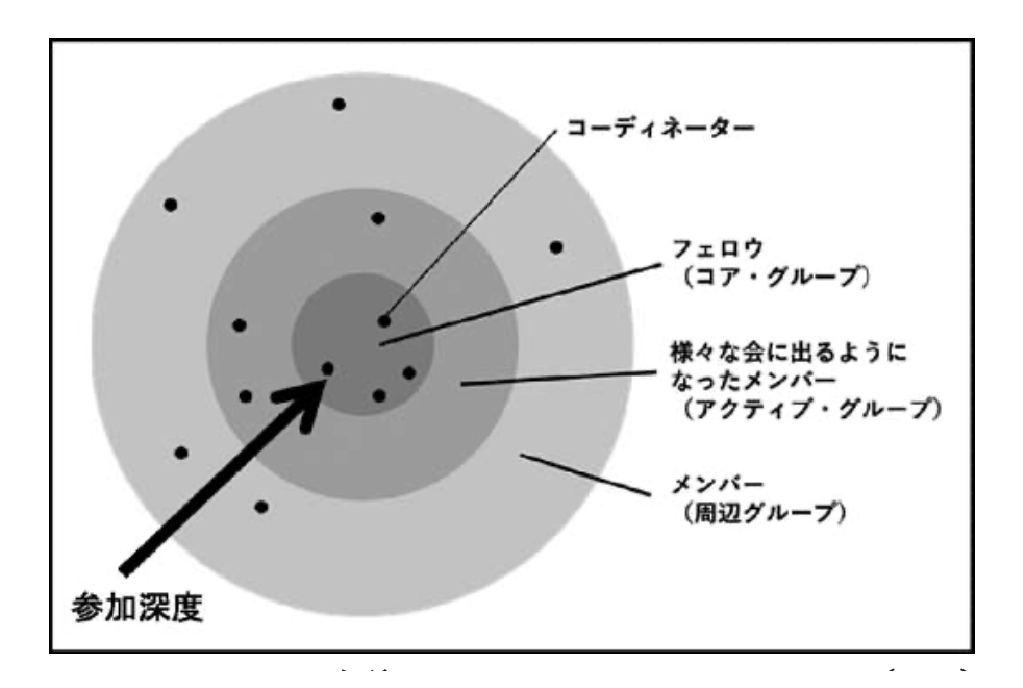
\includegraphics[width=0.5\textwidth]{img/cop.eps}
  \caption{実践共同体のイメージ図}
  \label{cop}
\end{figure}
正統的周辺参加とは,学習を成員がある実践共同体に加わり,
技能の獲得と成員のアイデンティティの発達を達成していくその動きとして捉える概念のことである.図1の周辺グループがそれにあたる.


加えて,正統的周辺参加として実践共同体に加わったその成員が,
その実践共同体内でどのような参加の過程を辿るかについては,
軌跡(Trajectory)という概念で表す.
ディスコースとは,実践共同体に共有される話し手のミクロな会話から
マクロな価値観まで含む文化のことを意味する\cite{discourse}.
\begin{figure}[h]
  \centering
  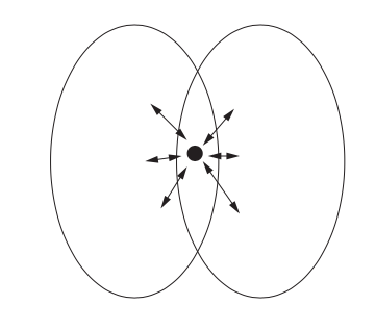
\includegraphics[width=0.5\textwidth]{img/overlap.eps}
  \caption{異なる実践共同体の協働のイメージ図}
  \label{overlap}
\end{figure}


布置とは,成員は単一の実践共同体のみに参加するものではなく,
複数の実践共同体に参加することを踏まえて,複数の実践共同体における
成員の振る舞いを捉える概念である.
松本\cite{Matsumoto}が作成した異なる実践共同体の重なりのイメージを図\ref{overlap}に示す.




実践共同体の概念は
学習という側面に関して多くの研究で効果が指摘されているが,
異なる実践共同体の関係構築のあり方と開発されるアプリへの影響についての
研究は著者が知る限りあまり行われていない.
しかし,上野\cite{uenoArt}が示すように人工物は,
様々な組織間やコミュニティ間の調停,交渉の産物として形成されている.


そのため,人工物のデザインとはコミュニティのデザインであると述べているように,
実践共同体の概念を用いた分析は学習以外にも焦点を向ける有用性があると考えられる.
上記の理由から,実践共同体の概念を通して,
異なる背景を持つメンバ同士の関係のあり方が
アプリのデザインにどのよう影響しているかを分析する手法は有効であると考える.

%3
\section{アプリ開発におけるPBLの実践共同体の概念による分析}
\label{previous-research-pbl}

著者らのこれまでの研究は,情報学部情報学科(以下,情報学科と表記する)と
人文学部国際関係学科(以下,国際学科と表記する)が学部横断による
PBL型授業を対象に分析が行われた.
観察対象のPBL型授業のテーマは,「地域観光を促進するアプリの開発」である.
情報学科と国際学科を異なる実践共同体として捉え,
複数の実践共同体の関係構築のあり方が開発されアプリのUIに
どのように影響しているかについて,分析を行っている.

国際学科と情報学科のそれぞれの実践共同体は,目的とする専門性や実践が異なる.
研究対象のPBL授業に参加する国際学科の学生は
英語でのプレゼンテーションが主な実践であり,
情報学科の学生はプログラミングやアプリ開発が主な実践となる.
 

PBL授業では,アプリの実装が完了した後で,
英語での成果発表という順番になるため,
異なる実践をもつ両学科の学生が
積極的にプロジェクトに参加する時期に齟齬がおきる傾向がみられた.


プロジェクトの前半はアプリ開発が主な作業となるため,
技術それ自体に価値を置く情報学科が積極的に参加し,
アプリ開発に携わった経験がほとんどない国際学科の学生は観察を主とした参加の態度になる.
これはアプリ開発という実践共同体に正統的周辺参加しているといえる.
他方,プロジェクト後半になると,アプリの成果発表があるため,
国際学科の学生がプロジェクトに積極的に参加し,
情報学科の学生が正統的周辺参加の態度を取る傾向が見られた.

それぞれ異なる実践共同体が築く関係のあり方として,
自分の専門性に関わるタスクしか関心を向けないという分業的な関係か
,または,自分の専門を超えて一緒に作業を行う時間を設ける協働的な
関係を築くかに分かれる.


分業的な関係のあり方でアプリ開発を進めた際,
タスクをこなす際に,部分最適化する傾向があり
制作された成果物は,異なる実践共同体の専門を組み合せるにとどまっていた.

他方,協働的な関係のあり方でアプリ開発を進めた際には,
短期的には非効率的に見えても,
アプリ開発の過程に
異なる実践共同体の実践,つまり,
プログラミング書いている最中の意味の交渉や目的の修正や共有が行われ,
お互いの専門性を融合して成果物を作成することを可能にした.
研究結果として,プロジェクトメンバの関係構築の在り方が分業的関係か協働的関係に応じて、
各プロジェクトメンバが所有する知識や技術といったリソースが
その人間関係のあり方に相応して開発プロセスに影響し、
アプリの機能やUIに現れるという示唆を得た.


本研究が開発したシステムは,アプリ開発支援システムとして,
異分野横断的なアプリ開発において,
異なる実践共同体が協働的な関係構築を行うことで,
お互いの実践を融合させてアプリ開発を支援することを目的としたシステムである.
使用場面として,ソフトウェアの開発手法の一つである
アジャイル開発に活用されることを想定している.
アジャイル開発とは機能単位の小さなサイクルで,
設計・開発・テストの工程を繰り返すことにより,
様々な状況の変化に対応しながら開発を進めていく手法である.
状況の変化に対応するため,
日毎にdaily scrumと呼ばれる短い時間での進捗の共有と反省を行う
打ち合わせの時間が設けられている.
開発したシステムはdaily scrumに活用されることが想定されており,
アプリ開発の要件から実装までを機能中心に組み立てるのではなく、
参加者それぞれの関心やスタンスを調整し
その関係のあり方そのものからデザインすることを可能にすることが期待されている.


% アプリ開発支援ソフトウェアは,実践共同体の概念を参考に設計されている.
% \begin{enumerate}
%     「正統的周辺参加」をTrelloの カードの移動,プロジェクトのタスクがどの共同体に属しいてるかをTrelloのラベル機能を用 いて表す.
% \end{enumerate}

\section{実践共同体の可視化システムについて}
\label{system-map}

本研究における可視化システムは,
Atlassian社が提供するタスク管理サービスTrello\cite{trello}と連携して動作する.
Trelloは,タスクの情報をカード,
タスクの状態をボードとして管理するサービスである.
利用者は,タスクを実行した際に,
カードを次のボードに移動させる.
これにより,プロジェクトメンバ間でタスクの進捗状況を共有することができる.
また,Trelloでは,カードに複数人の作業担当者を設定することが可能である.
そこで,本システムでは,
同じカードに割り振られた作業担当者は,
協働でタスクを行ったという前提で,
Trello上でのカードの移動履歴を利用することで,
プロジェクトメンバが協働で作業を行っている様子を可視化した.

% 従来の概念図と,本システムによる可視化の比較
% MEMO: N個のベン図は表現可能
% https://nunuki.hatenablog.com/entry/2017/12/31/175302
従来までの実践共同体とメンバの関係性は,
図\ref{cop}と図\ref{overlap}で示したように,
実践共同体とメンバを,
領域と要素のように表現されてきた.
% しかし,実践共同体とプロジェクトメンバの関係性を可視化する際に,
% 図\ref{cop}の様な表現を採用することを考えると,
% 実践共同体の中心と,メンバの距離を表すことはできるが,
% メンバ間の距離や,
% メンバ間のなす角が余計な情報として表されてしまう.
% もし,距離やなす角によって,
% 協働でタスクを行った回数などを表すとしても,
% メンバが四人以上のプロジェクトを対象とした場合に,
% 二次元平面で全てのメンバの関係性を表現することはできない.
しかし,実践共同体とプロジェクトメンバの関係性を可視化する際に,
図\ref{cop}の様な表現を採用することを考えると,
参加深度と同時に,
メンバ同士の関係性を距離によって表現することは困難だと考えられる.
また,布置を可視化する際に,
図\ref{overlap}の様な表現を採用することを考えた場合にも,
3つ以上の実践共同体を表現しようとした際に,
閉曲線が複雑化してしまう可能性が考えられる.
そこで,本研究では,
プロジェクトメンバをノード,
プロジェクトメンバが協働でタスクを行った履歴をエッジとすることで,
プロジェクトの状況をネットワーク構造によって表現した.
これにより,複雑なメンバの関係性や,
異なる実践共同体間の関係性を観察することを可能にした.
本システムによって可視化したプロジェクトメンバの関係性を,
図\ref{cop-map-graph}に示す.

\begin{figure}[h]
  \centering
  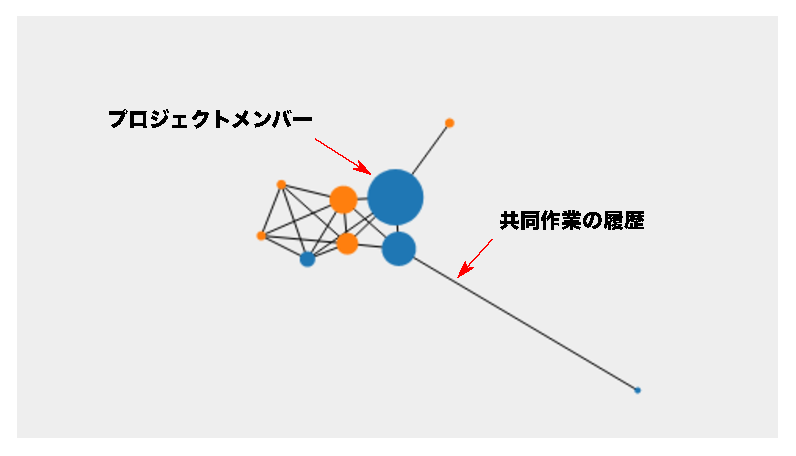
\includegraphics[width=0.5\textwidth]{img/cop-map-graph.eps}
  \caption{本システムによってプロジェクトメンバの関係性を可視化した様子}
  \label{cop-map-graph}
\end{figure}

本システムでは,ノードのレイアウト手法として,力学モデルを採用している.
また,協働でタスクを行った回数によってエッジの強度を変化させることで,
多くのタスクを協働で行うほど,
ノード間の距離は近くなるように配置される.
これにより,頻繁に協働でタスクを行っているプロジェクトメンバを確認することができる.
また,そのプロジェクトメンバが異なる実践共同体に所属していた場合に,
異なる実践共同体の間で,協働的にタスクが行われているかを観察することができる.
本システムによって可視化された,
協働で行われたタスクの様子を図\ref{cop-map-task}に示す.

\begin{figure}[h]
  \centering
  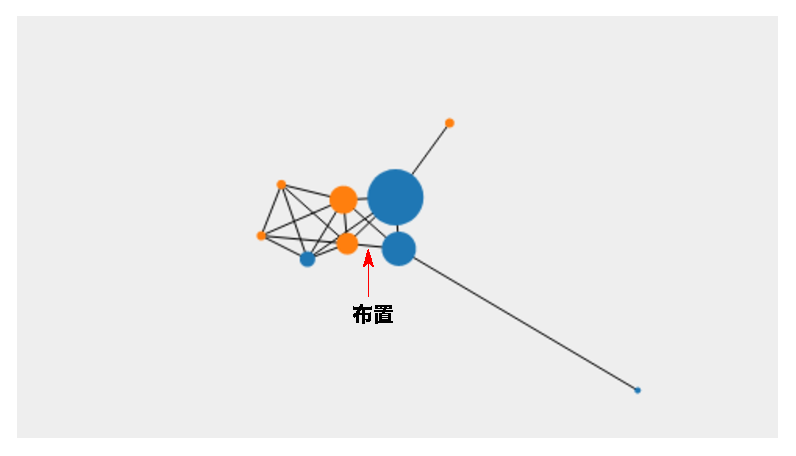
\includegraphics[width=0.5\textwidth]{img/cop-map-task.eps}
  \caption{本システムによって可視化された協働で行われたタスク}
  \label{cop-map-task}
\end{figure}

また,プロジェクトメンバの所属先によってノードの色を変化させることで,
異なる実践共同体に所属するプロジェクトメンバが,
協働でタスクを行っている様子を観察することを可能にしている.
これにより,異なる色のノードがエッジでつながっている様子から,
布置を観察することができる.
本システムによって観察される布置の例を,
図 \ref{cop-map-overlap}に示す.

\begin{figure}[h]
  \centering
  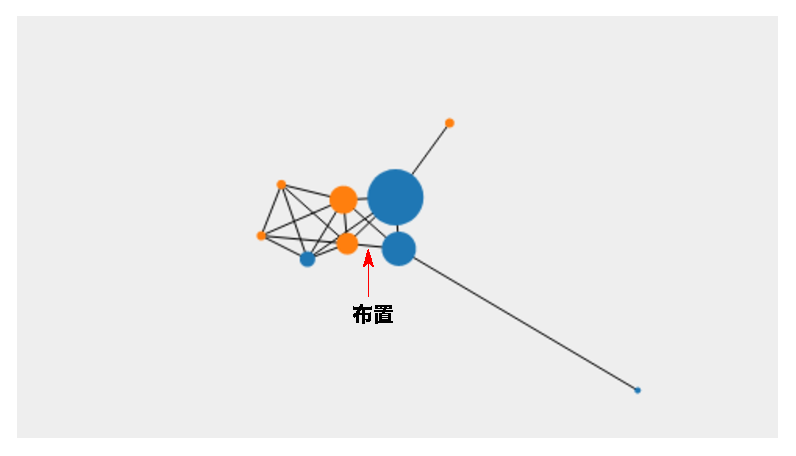
\includegraphics[width=0.5\textwidth]{img/cop-map-overlap.eps}
  \caption{本システムによって可視化された布置}
  \label{cop-map-overlap}
\end{figure}

さらに,タスクを行った回数の合計値によってノードの大きさを変化させている.
これにより,プロジェクトメンバが正統的周辺参加である可能性を観察することが可能である.
その一例として,ノードは小さいが,他のノードとの繋がりが見られる場合が挙げられる.
この場合は,観察対象となるプロジェクトメンバは,
タスクを行った回数は少ないが,
リソースへのアクセスが可能な状態だと考える事ができる.
本システムによって,
観察される正統的周辺参加である可能性のあるプロジェクトメンバを図\ref{cop-map-lpp}に示す.

\begin{figure}[h]
  \centering
  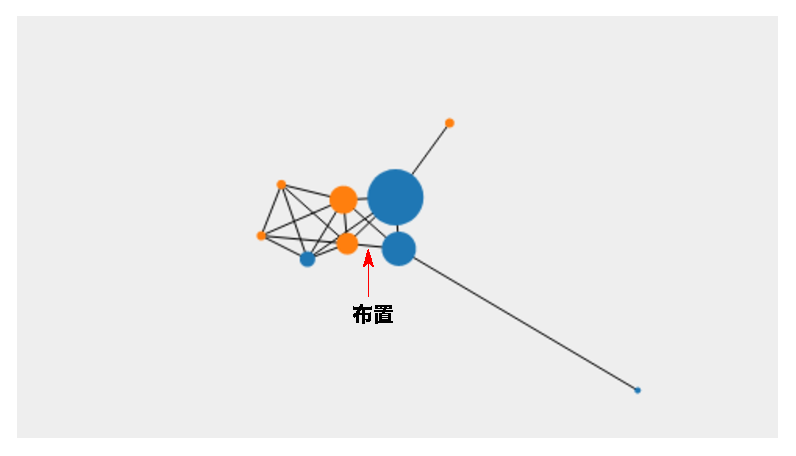
\includegraphics[width=0.5\textwidth]{img/cop-map-lpp.eps}
  \caption{本システムによって観察される正統的周辺参加である可能性のあるプロジェクトメンバ}
  \label{cop-map-lpp}
\end{figure}

以上のネットワーク構造を,プロジェクトの時系列順に変化させることで,
プロジェクトメンバの関係性の変化を観察することを可能にしている.
これにより,ノードの軌跡から,
進行状況によって変化していく,
プロジェクトメンバの軌跡を観察することを可能にしている.
本システムによって観察されるプロジェクトメンバの軌跡を,
図\ref{cop-map-trajectory}に示す.

\begin{figure}[h]
  \centering
  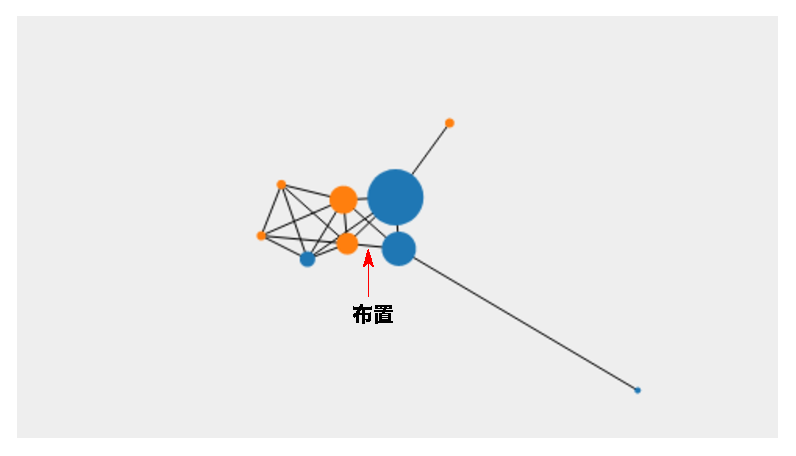
\includegraphics[width=0.5\textwidth]{img/cop-map-trajectory.eps}
  \caption{本システムによって観察されるプロジェクトメンバの軌跡}
  \label{cop-map-trajectory}
\end{figure}

また,本システムではインタラクティブにデータを観察することが可能である.
本システムで可能なインタラクションは,
ノードのドラッグアンドドロップと,ノードへのマウスオーバーである.
ノードをドラッグアンドドロップすることによって,
ネットワークのレイアウトを調整することが可能である.
また,メンバの詳細情報を確認する際には,
ノードにマウスオーバーすることで,
そのノードに対応するユーザ名を確認することが可能である.
これらのインタラクションにより,
より詳細にプロジェクトメンバの関係性を観察することが可能である.
インタラクションによって詳細情報を表示している様子を,
図\ref{cop-map-detail}に示す.

\begin{figure}[h]
  \centering
  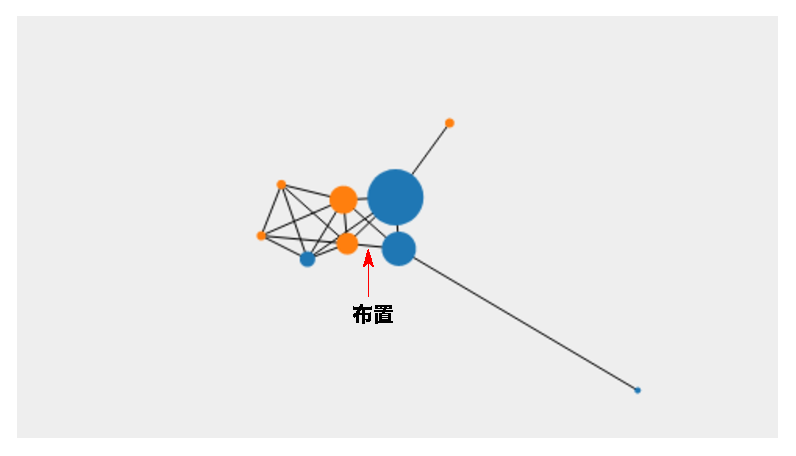
\includegraphics[width=0.5\textwidth]{img/cop-map-detail.eps}
  \caption{インタラクションによって詳細情報を表示している様子}
  \label{cop-map-detail}
\end{figure}

%4
\section{今後の展望}

本研究で開発したシステムは,2021年度9月より実施される学部横断型PBLのアプリ開発を
行う際に使用される予定である.開発したシステムから,
メンバの背景と行為やメンバ間の交渉に着目し,
アプリの機能やUIがどのように決定されていくか 分析する予定である.
加えてアプリ開発支援ソフトウェアがアプリ開発の過程にどのように影響を及ぼすかまで含めて分析を行う.

% 遠藤が実装したい内容ついての記述

%5
\section{おわりに}

% 今後の展望と終わりにまとめてしまってもよい?

\section*{謝辞}
シングルブラインド査読のため,謝辞は入れた状態で投稿する.
謝辞の例:本研究はJSPS科研費 JP12345678の助成を受けたものです.


%%
%%	参考文献
%%
% \begin{thebibliography}{1}
% \end{thebibliography}

\section{てすと}

てすとてすとてすとてすとてすとてすとてすとてすとてすとてすと.
てすとてすとてすとてすとてすとてすとてすとてすとてすとてすと.
てすとてすとてすとてすとてすとてすとてすとてすとてすとてすと.
てすとてすとてすとてすとてすとてすとてすとてすとてすとてすと.
てすとてすとてすとてすとてすとてすとてすとてすとてすとてすと.
てすとてすとてすとてすとてすとてすとてすとてすとてすとてすと.
てすとてすとてすとてすとてすとてすとてすとてすとてすとてすと.
てすとてすとてすとてすとてすとてすとてすとてすとてすとてすと.
てすとてすとてすとてすとてすとてすとてすとてすとてすとてすと.
てすとてすとてすとてすとてすとてすとてすとてすとてすとてすと.
てすとてすとてすとてすとてすとてすとてすとてすとてすとてすと.
てすとてすとてすとてすとてすとてすとてすとてすとてすとてすと.
てすとてすとてすとてすとてすとてすとてすとてすとてすとてすと.
てすとてすとてすとてすとてすとてすとてすとてすとてすとてすと.
てすとてすとてすとてすとてすとてすとてすとてすとてすとてすと.
てすとてすとてすとてすとてすとてすとてすとてすとてすとてすと.


文章量が増えると,本文と未来ビジョンが重なるため,重ならないように文章量を調整すること.

\balance %最後の高さを揃えるために必要 (2012/9/27:watanabe, Igarashi)
\bibliographystyle{jwiss}
\bibliography{sample}



%%%%%%%%%%%%%%%%%%%%%%%%%%%%%%%%%%%%%%%%%%%%%%%%%%%%%%%%%%%%%%%%%%%%%
%%%%%%%%%%%%%%%%%%%%%%%%%%%%%%%%%%%%%%%%%%%%%%%%%%%%%%%%%%%%%%%%%%%%%
%% WISS2012では,「未来ビジョン」は以下のように,本文と同様の2段組形式で記載する.
%% 図を用いても良いが,枠のサイズ(縦93mm)を変更してはならない.
%% (WISS2010では,縦118mmでしたのでご注意下さい)

\begin{figure*}[!b]
\setlength{\unitlength}{1mm}\fboxrule=0.5pt

\vspace{-93mm} %% 未来ビジョンの枠が下がってしまうのを防ぐ WIS2012 カメラレディテンプレで追加  (2012/9/27:watanabe, Igarashi)

% 未来ビジョンの枠の描画
\begin{center}
\framebox[0.95\textwidth]{
\begin{minipage}{0mm}\begin{picture}(0,91)(0,0)\end{picture}\end{minipage}
}
\end{center}
\vspace*{-93mm}	% 未来ビジョンの枠の縦幅分だけ戻す

% 未来ビジョンの内容
\newbox\FUTURE
\setbox\FUTURE=\vbox{
\begin{minipage}[b]{0.9\textwidth}
\begin{multicols}{2}	% 二段組にする
\section*{未来ビジョン}
\setlength{\parindent}{10pt}	% 段落先頭の字下げ

% % % % % % % % % % % % % % % % % % % % % % % % % % % % % %
%	   未来ビジョンは,下記に記入して下さい		  %
% % % % % % % % % % % % % % % % % % % % % % % % % % % % % %

\vspace*{-1mm}

% フォントサイズ指定
\normalsize
%\large
%\small\setlength{\baselineskip}{12pt}
%\footnotesize\setlength{\baselineskip}{12pt}

(本行を含む下記の説明を削除してから,記入すること.)

未来ビジョンについては,必須とせず任意とする.論文本体とは別
に,「この研究はどういう未来を切り拓くのか」について,著者の視点からア
ピールしたい点があれば,このような欄を設けて設けて自由に議論してよい.
例えば,「こういう未来社会が到来して欲しいから,我々の研究でこう貢献
していきたい」,「主張が大きすぎて本文中では書きにくかったが,この研究
は,実はこういう気持ちで研究している」,「現在の実装では,小さいトピック
であるかのように誤解を招きやすいが,本当はこういう大きなことを狙って,そ
の第一歩として研究に取り組んでいる」のように,研究の未来,魅力を語る場と
して利用できる.大きさや形状はこのサンプルを目安とするが,この枠内であればある程
度改変してもよいものとする.

てすとてすとてすとてすとてすとてすとてすとてすとてすとてすと.てすとてすとてすとてすとてすとてすとてすとてすとてすとてすと.てすとてすとてすとてすとてすとてすとてすとてすとてすとてすと.てすとてすとてすとてすとてすとてすとてすとてすとてすとてすと.てすとてすとてすとてすとてすとてすとてすとてすとてすとてすと.てすとてすとてすとてすとてすとてすとてすとてすとてすとてすと.てすとてすとてすとてすとてすとてすとてすとてすとてすとてすと.
%% 文章を補う図表を利用してもよい.
\vspace*{5mm}
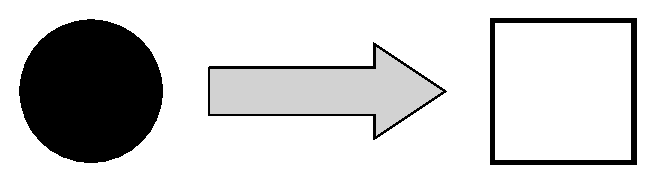
\includegraphics[width=0.95\columnwidth]{vision.eps}
% % % % % % % % % % % % % % % % % % % % % % % % % % % % % %
%	   未来ビジョンは,上記に記入して下さい		  %
% % % % % % % % % % % % % % % % % % % % % % % % % % % % % %

\end{multicols}
\end{minipage}
}

% 未来ビジョンの内容の描画
\newlength{\FUTUREHT}
\setlength{\FUTUREHT}{\the\ht\FUTURE}	% 未来ビジョンの内容の縦幅保存
%\typeout{\the\wd\FUTURE}
%\typeout{\the\ht\FUTURE}
\hspace*{0.045\textwidth}	% 未来ビジョンの内容の横位置調整
\box\FUTURE
%\typeout{\the\FUTUREHT}
\vspace*{-\the\FUTUREHT}	% 未来ビジョンの内容の縦幅分だけ戻す
\vspace*{-10.9mm}		% 微調整

% 未来ビジョンの枠の領域の再確保(これがないと枠が下に沈み込む)
\begin{center}
\fboxrule=0pt
%\fboxrule=2pt	% デバッグ用: コメントアウトをやめて,同じ位置に枠が出るか?
\framebox[0.9\textwidth]{
\begin{minipage}{0mm}\begin{picture}(0,91)(0,0)\end{picture}\end{minipage}
}
\end{center}
\end{figure*}

%%%%%%%%%%%%%%%%%%%%%%%%%%%%%%%%%%%%%%%%%%%%%%%%%%%%%%%%%%%%%%%%%%%%%
%%%%%%%%%%%%%%%%%%%%%%%%%%%%%%%%%%%%%%%%%%%%%%%%%%%%%%%%%%%%%%%%%%%%%
\end{document}
